% Copyright 2006 by Till Tantau
%
% This file may be distributed and/or modified
%
% 1. under the LaTeX Project Public License and/or
% 2. under the GNU Free Documentation License.
%
% See the file doc/generic/pgf/licenses/LICENSE for more details.


\section{Automata Drawing Library}

\begin{tikzlibrary}{automata}
    This packages provides shapes and styles for drawing finite state automata
    and Turing machines.
\end{tikzlibrary}
%
\begin{codeexample}[setup code,hidden]
    \usetikzlibrary{automata}
\end{codeexample}


\subsection{Drawing Automata}

The automata drawing library is intended to make it easy to draw finite
automata and Turing machines. It does not cover every situation imaginable, but
most finite automata and Turing machines found in text books can be drawn in a
nice and convenient fashion using this library.

To draw an automaton, proceed as follows:
%
\begin{enumerate}
    \item For each state of the automaton, there should be one node with the
        option |state|.
    \item To place the states, you can either use absolute positions or
        relative positions, using options like |above| or |right|.
    \item Give a unique name to each state node.
    \item Accepting and initial states are indicated by adding the options
        |accepting| and |initial|, respectively, to the state nodes.
    \item Once the states are fixed, the edges can be added. For this, the
        |edge| operation is most useful. It is, however, also possible to add
        edges after each node has been placed.
    \item For loops, use the |edge [loop]| operation.
\end{enumerate}

Let us now see how this works for a real example. Let us consider a
nondeterministic four state automaton that checks whether an input contains the
sequence $0^*1$ or the sequence $1^*0$.
%
\begin{codeexample}[preamble={\usetikzlibrary{positioning}}]
\begin{tikzpicture}[shorten >=1pt,node distance=2cm,on grid,auto]
  \draw[help lines] (0,0) grid (3,2);

  \node[state,initial]  (q_0)                      {$q_0$};
  \node[state]          (q_1) [above right=of q_0] {$q_1$};
  \node[state]          (q_2) [below right=of q_0] {$q_2$};
  \node[state,accepting](q_3) [below right=of q_1] {$q_3$};

  \path[->] (q_0) edge              node        {0} (q_1)
                  edge              node [swap] {1} (q_2)
            (q_1) edge              node        {1} (q_3)
                  edge [loop above] node        {0} ()
            (q_2) edge              node [swap] {0} (q_3)
                  edge [loop below] node        {1} ();
\end{tikzpicture}
\end{codeexample}


\subsection{States With and Without Output}

The |state| style actually just ``selects'' a default underlying style. Thus,
you can define multiple new complicated state style and then simply set the
|state| style to your given style to get the desired kind of styles.

By default, the following state styles are defined:
%
\begin{stylekey}{/tikz/state without output}
    This node style causes nodes to be drawn as circles. Also, this style calls
    |every state|.
\end{stylekey}

\begin{stylekey}{/tikz/state with output}
    This node style causes nodes to be drawn as split circles, that is, using
    the |circle split| shape. In the upper part of the shape you have the name
    of the style, in the lower part the output is placed. To specify the
    output, use the command |\nodepart{lower}| inside the node. This style also
    calls |every state|.
    %
\begin{codeexample}[]
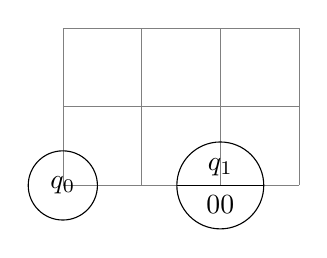
\begin{tikzpicture}
  \draw[help lines] (0,0) grid (3,2);

  \node[state without output] {$q_0$};

  \node[state with output] at (2,0) {$q_1$ \nodepart{lower} $00$};
\end{tikzpicture}
\end{codeexample}
    %
\end{stylekey}

\begin{stylekey}{/tikz/state (initially state without output)}
    You should redefine it to something else, if you wish to use states of a
    different nature.
\begin{codeexample}[]
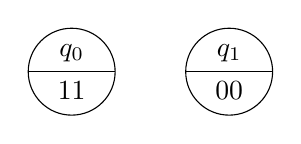
\begin{tikzpicture}[state/.style=state with output]
  \node[state]          {$q_0$ \nodepart{lower} $11$};
  \node[state] at (2,0) {$q_1$ \nodepart{lower} $00$};
\end{tikzpicture}
\end{codeexample}
    %
\end{stylekey}

\begin{stylekey}{/tikz/every state (initially \normalfont empty)}
    This style is used by |state with output| and also by
    |state without output|. By default, it does nothing, but you can use it to
    make your state look more fancy:
    %
\begin{codeexample}[preamble={\usetikzlibrary{arrows,positioning}}]
\begin{tikzpicture}[shorten >=1pt,node distance=2cm,on grid,>=stealth',
    every state/.style={draw=blue!50,very thick,fill=blue!20}]

  \node[state,initial]  (q_0)                      {$q_0$};
  \node[state]          (q_1) [above right=of q_0] {$q_1$};
  \node[state]          (q_2) [below right=of q_0] {$q_2$};

  \path[->] (q_0) edge              node [above left]  {0} (q_1)
                  edge              node [below left]  {1} (q_2)
            (q_1) edge [loop above] node               {0} ()
            (q_2) edge [loop below] node               {1} ();
\end{tikzpicture}
\end{codeexample}
    %
\end{stylekey}


\subsection{Initial and Accepting States}

The styles |initial| and |accepting| are similar to the |state| style as they
also just select an ``underlying'' style, which installs the actual settings
for initial and accepting states.

Let us start with the initial states.
%
\begin{stylekey}{/tikz/initial (initially initial by arrow)}
    This style is used to draw initial states.
\end{stylekey}

\begin{stylekey}{/tikz/initial by arrow}
    This style causes an arrow and, possibly, some text to be added to the
    node. The arrow points from the text to the node. The node text and the
    direction and the distance can be set using the following key:
    %
    \begin{key}{/tikz/initial text=\meta{text} (initially start)}
        This key sets the text to be used. Use an empty text to suppress all
        text.
    \end{key}
    %
    \begin{key}{/tikz/initial where=\meta{direction} (initially left)}
        Set the place where the text should be shown. Allowed values are
        |above|, |below|, |left|, and |right|.
    \end{key}
    %
    \begin{key}{/tikz/initial distance=\meta{distance} (initially 3ex)}
        Sets the length of the arrow leading from the text to the state node.
    \end{key}
    %
    \begin{stylekey}{/tikz/every initial by arrow (initially \normalfont empty)}
        This style is executed at the beginning of every path that contains the
        arrow and the text. You can use it to, say, make the text red or
        whatever.
    \end{stylekey}
    %
\begin{codeexample}[]
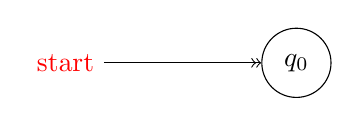
\begin{tikzpicture}[every initial by arrow/.style={text=red,->>}]
  \node[state,initial,initial distance=2cm] {$q_0$};
\end{tikzpicture}
\end{codeexample}
    %
\end{stylekey}

\begin{stylekey}{/tikz/initial above}
    This is a shorthand for |initial by arrow,initial where=above|.
\end{stylekey}

\begin{stylekey}{/tikz/initial below}
    Works similarly to the previous option.
\end{stylekey}

\begin{stylekey}{/tikz/initial left}
    Works similarly to the previous option.
\end{stylekey}

\begin{stylekey}{/tikz/initial right}
    Works similarly to the previous option.
\end{stylekey}

\begin{stylekey}{/tikz/initial by diamond}
    This style uses a diamond to indicate an initial node.
\end{stylekey}

For the accepting states, the situation is similar: There is also an
|accepting| style that selects the way accepting states are rendered. There are
now two options: First, |accepting by arrow|, which works the same way as
|initial by arrow|, only with the direction of arrow reversed, and
|accepting by double|, where accepting states get a double line around them.

\begin{stylekey}{/tikz/accepting (initially accepting by double)}
    This style is used to draw accepting states.  You can replace this by the
    style |accepting by arrow| to get accepting states with an arrow leaving
    them.
\end{stylekey}

\begin{stylekey}{/tikz/accepting by double}
    This style causes a double line to be drawn around a state.
\end{stylekey}

\begin{stylekey}{/tikz/accepting by arrow}
    This style causes an arrow and, possibly, some text to be added to the
    node. The arrow points to the text from the node.

    The same options as for initial states can be used, only with |initial|
    replaced by |accepting|:
    %
    \begin{key}{/tikz/accepting text=\meta{text} (initially \normalfont empty)}
        This key sets the text to be used.
    \end{key}
    %
    \begin{key}{/tikz/accepting where=\meta{direction} (initially right)}
        Set the place where the text should be shown. Allowed values are
        |above|, |below|, |left|, and |right|.
    \end{key}
    %
    \begin{key}{/tikz/initial distance=\meta{distance} (initially 3ex)}
        Sets the length of the arrow leading from the text to the state
        node.
    \end{key}
    %
    \begin{stylekey}{/tikz/every accepting by arrow (initially \normalfont empty)}
        Executed at the beginning of every path that contains the arrow and the
        text.
    \end{stylekey}
    %
\begin{codeexample}[preamble={\usetikzlibrary{arrows,positioning}}]
\begin{tikzpicture}
  [shorten >=1pt,node distance=2cm,on grid,>=stealth',initial text=,
   every state/.style={draw=blue!50,very thick,fill=blue!20},
   accepting/.style=accepting by arrow]

  \node[state,initial]  (q_0)                      {$q_0$};
  \node[state]          (q_1) [above right=of q_0] {$q_1$};
  \node[state]          (q_2) [below right=of q_0] {$q_2$};
  \node[state,accepting](q_3) [below right=of q_1] {$q_3$};

  \path[->] (q_0) edge              node [above left]  {0} (q_1)
                  edge              node [below left]  {1} (q_2)
            (q_1) edge              node [above right] {1} (q_3)
                  edge [loop above] node               {0} ()
            (q_2) edge              node [below right] {0} (q_3)
                  edge [loop below] node               {1} ();
\end{tikzpicture}
\end{codeexample}
    %
\end{stylekey}

\begin{stylekey}{/tikz/accepting above}
    This is a shorthand for |accepting by arrow,accepting where=above|.
\end{stylekey}

\begin{stylekey}{/tikz/accepting below}
    Works similarly to the previous option.
\end{stylekey}

\begin{stylekey}{/tikz/accepting left}
    Works similarly to the previous option.
\end{stylekey}

\begin{stylekey}{/tikz/accepting right}
    Works similarly to the previous option.
\end{stylekey}


\subsection{Examples}

In the following example, we once more typeset the automaton presented in the
previous sections. This time, we use the following rule for accepting/initial
state: Initial states are red, accepting states are green, and normal states
are orange. Then, we must find a path from a red state to a green state.
%
\begin{codeexample}[preamble={\usetikzlibrary{arrows,positioning,shadows}}]
\begin{tikzpicture}[shorten >=1pt,node distance=2cm,on grid,>=stealth',thick,
    every state/.style={fill,draw=none,orange,text=white,circular drop shadow},
    accepting/.style  ={green!50!black,text=white},
    initial/.style    ={red,text=white}]

  \node[state,initial]  (q_0)                      {$q_0$};
  \node[state]          (q_1) [above right=of q_0] {$q_1$};
  \node[state]          (q_2) [below right=of q_0] {$q_2$};
  \node[state,accepting](q_3) [below right=of q_1] {$q_3$};

  \path[->] (q_0) edge              node [above left]  {0} (q_1)
                  edge              node [below left]  {1} (q_2)
            (q_1) edge              node [above right] {1} (q_3)
                  edge [loop above] node               {0} ()
            (q_2) edge              node [below right] {0} (q_3)
                  edge [loop below] node               {1} ();
\end{tikzpicture}
\end{codeexample}

The next example is the current candidate for the five-state busiest beaver:
%
\begin{codeexample}[preamble={\usetikzlibrary{arrows,positioning}}]
\begin{tikzpicture}[->,>=stealth',shorten >=1pt,%
                    auto,node distance=2cm,on grid,semithick,
                    inner sep=2pt,bend angle=45]
  \node[initial,state] (A)                    {$q_a$};
  \node[state]         (B) [above right=of A] {$q_b$};
  \node[state]         (D) [below right=of A] {$q_d$};
  \node[state]         (C) [below right=of B] {$q_c$};
  \node[state]         (E) [below=of D]       {$q_e$};

  \path [every node/.style={font=\footnotesize}]
        (A) edge              node {0,1,L} (B)
            edge              node {1,1,R} (C)
        (B) edge [loop above] node {1,1,L} (B)
            edge              node {0,1,L} (C)
        (C) edge              node {0,1,L} (D)
            edge [bend left]  node {1,0,R} (E)
        (D) edge [loop below] node {1,1,R} (D)
            edge              node {0,1,R} (A)
        (E) edge [bend left]  node {1,0,R} (A);
\end{tikzpicture}
\end{codeexample}


%%% Local Variables:
%%% mode: latex
%%% TeX-master: "pgfmanual-pdftex-version"
%%% End:
